\section{Session 5 - Sequential circuit and unit}
\vspace{-15pt}\noindent\rule{\textwidth}{0.1pt}\vspace{-10pt}
    \subsection{Notes}
    {\color{hwSolution}
    \subsection*{Another method to generate delayed paluse - without losing its length}
        \begin{center}\begin{tikzpicture}
% CHIP 2 (Y+0.0)
    \draw[black,thick]
      (-1.2,2.4)--(-1.2,0.0)
    --( 1.2,0.0)--( 1.2,2.4)
    --cycle;
    % Left Side
    \draw[black,thick, -] (-1.2,1.6) node[right]{$A$}
    -- (-2.0,1.6) node[left]{$V_{DD}$};
    \draw[black,thick,o-] (-1.2, 0.8) node[right]{$B$}
    -- (-2.0,0.8) node[left]{\textit{GND}};
    % Right Side
    \draw[black,thick, -] ( 1.2, 1.6) node[left]{$Q$}
    -- ( 2.0, 1.6);
    \draw[black,thick,o-] ( 1.2, 0.8) node[left]{$\bar{Q}$}
    -- ( 1.4, 0.8);
    % Top Side
    \draw[black,thick, -] (-0.4, 2.4) node[below]{$C_X$}
    -- (-0.4, 3.0);
    \draw[black,thick, -] ( 0.4, 2.4) node[below]{$R_X$}
    -- ( 0.4, 3.0);
    % Bottom Side
    \draw[black,thick,o-*] ( 0.0, 0.0) node[above]{$C_{L}$}
    -- ( 0.0,-0.6) -- ( 1.8,-0.6);
    % C/R
    \draw[black,thick, -]
        % Capacitor
        (-0.4, 3.0) -- (-0.1, 3.0)
        ( 0.4, 3.0) -- ( 0.1, 3.0)
        ( 0.1, 3.2) -- ( 0.1, 2.8)
        (-0.1, 3.2) -- (-0.1, 2.8)
        ( 0.0, 3.2) node[above]{$C$}
        % Resistor
        ( 0.4, 3.0) -- ( 0.7, 3.0)
        ( 1.2, 3.0) -- ( 1.5, 3.0)
        ( 0.7, 3.1) -- ( 1.2, 3.1) -- ( 1.2, 2.9) -- ( 0.7, 2.9) -- cycle
        ( 0.95, 3.2) node[above]{$R$};
    \draw[black,thick,-*] ( 1.5, 3.0) -- ( 1.8, 3.0);
% CHIP 1 (Y+4.0)
    \draw[black,thick]
    (-1.2,2.4)--(-1.2,0.0)
  --( 1.2,0.0)--( 1.2,2.4)
  --cycle;
  % Left Side
  \draw[black,thick, -] (-1.2,1.6) node[right]{$A$}
  -- (-2.0,1.6) node[left]{$V_{DD}$};
  \draw[black,thick,o-] (-1.2, 0.8) node[right]{$B$}
  -- (-2.0,0.8) node[left]{\textit{GND}};
  % Right Side
  \draw[black,thick, -] ( 1.2, 1.6) node[left]{$Q$}
  -- ( 2.0, 1.6);
  \draw[black,thick,o-] ( 1.2, 0.8) node[left]{$\bar{Q}$}
  -- ( 1.4, 0.8);
  % Top Side
  \draw[black,thick, -] (-0.4, 2.4) node[below]{$C_X$}
  -- (-0.4, 3.0);
  \draw[black,thick, -] ( 0.4, 2.4) node[below]{$R_X$}
  -- ( 0.4, 3.0);
  % Bottom Side
  \draw[black,thick,o-*] ( 0.0, 0.0) node[above]{$C_{L}$}
  -- ( 0.0,-0.6) -- ( 1.8,-0.6);
  % C/R
  \draw[black,thick, -]
      % Capacitor
      (-0.4, 3.0) -- (-0.1, 3.0)
      ( 0.4, 3.0) -- ( 0.1, 3.0)
      ( 0.1, 3.2) -- ( 0.1, 2.8)
      (-0.1, 3.2) -- (-0.1, 2.8)
      ( 0.0, 3.2) node[above]{$C$}
      % Resistor
      ( 0.4, 3.0) -- ( 0.7, 3.0)
      ( 1.2, 3.0) -- ( 1.5, 3.0)
      ( 0.7, 3.1) -- ( 1.2, 3.1) -- ( 1.2, 2.9) -- ( 0.7, 2.9) -- cycle
      ( 0.95, 3.2) node[above]{$R$};
  \draw[black,thick,-*] ( 1.5, 3.0) -- ( 1.8, 3.0);
% Wire
\end{tikzpicture}\end{center}

        Functionality analysis:

        \begin{center}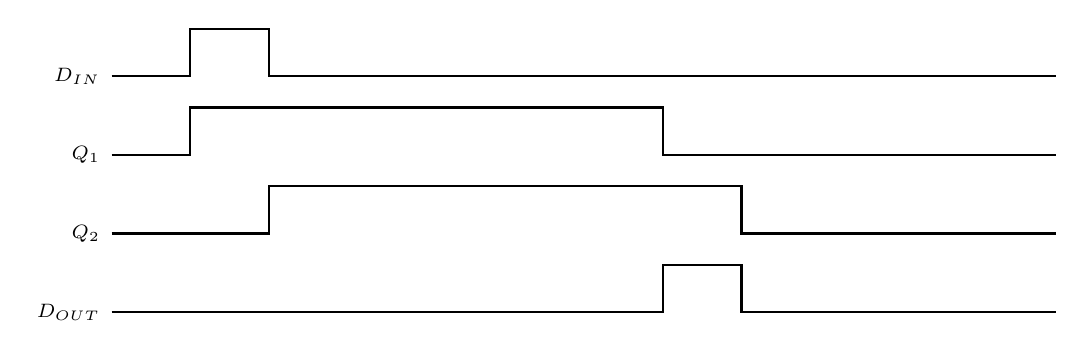
\begin{tikzpicture}
            \draw[black,thick]
                (0.0,3.0) node[left]{$_{D_{IN}}$}
                --(0.0,3.0)
                --(1.0,3.0)--(1.0,3.6)
                --(2.0,3.6)--(2.0,3.0)
                --(12.0,3.0);
            \draw[black,thick]
                (0.0,2.0) node[left]{$_{Q_{1}}$}
                --(0.0,2.0)
                --(1.0,2.0)--(1.0,2.6)
                --(7.0,2.6)--(7.0,2.0)
                --(12.0,2.0);
            \draw[black,thick]
                (0.0,1.0) node[left]{$_{Q_{2}}$}
                --(0.0,1.0)
                --(2.0,1.0)--(2.0,1.6)
                --(8.0,1.6)--(8.0,1.0)
                --(12.0,1.0);
            \draw[black,thick]
                (0.0,0.0) node[left]{$_{D_{OUT}}$}
                --(0.0,0.0)
                --(7.0,0.0)--(7.0,0.6)
                --(8.0,0.6)--(8.0,0.0)
                --(12.0,0.0);
        \end{tikzpicture}\end{center}
    }
    \subsection{Homework}
    \subsubsection{8.3 \textnormal{Analyze Logical function of the given circuit}.}
        \begin{center}\begin{tikzpicture}
    \def \HFH{10}
    \coordinate (DATA) at (5, 0);
    \draw[black]
        \foreach \x in {0,...,7}{
            (DATA)+({\x * 0.2},\HFH)--+({\x * 0.2},-\HFH)
        }
        (DATA)+(0.0,\HFH) node[above,left]{$D_7$}
        (DATA)+(1.4,\HFH) node[above,right]{$D_0$};
    \coordinate (ADDR) at (0, 0);
    \draw[black]
        \foreach \x in {2,...,11}{
            (ADDR)+({\x * 0.1},\HFH)--+({\x * 0.1},-\HFH)
        }
        (ADDR)+(0.0,\HFH) node[above,left]{$A_{11}$}
        (ADDR)+(1.1,\HFH) node[above,right]{$A_0$};
    % 24 Decoder
    \coordinate (C0) at (-4, 0);
    \draw[hwSolution,thick]
        (C0)+(-1,1.6) -- +(1,1.6) -- +(1,-1.6) -- +(-1,-1.6) -- cycle;
    \draw[black]
        (C0)+(-1.0, 0.8) node[right]{$A_0$} -- +(-1.4, 0.8)
        (C0)+(-1.0,-0.8) node[right]{$A_1$} -- +(-1.4,-0.8)
        (C0)+(-1.4, 0.8) -- +(-1.4,{\HFH-1.5}) -- (0.1,{\HFH-1.5}) -- (0.1,\HFH)
        (C0)+(-1.4,-0.8) -- +(-1.5,-0.8) -- +(-1.5,{\HFH-1.4}) -- (0.0,{\HFH-1.4}) -- (0.0,\HFH);
    \draw[hwSolution,thick,o-*] (C0)+( 1.0, 1.2) node[left] {$Y_0$} -- +( 1.4, 1.2) --  (-2.4, 1.2) -- (-2.4, 6.7) -- (-0.9, 6.7);
    \draw[hwSolution,thick,o-*] (C0)+( 1.0, 0.4) node[left] {$Y_1$} -- +( 1.4, 0.4) --  (-2.0, 0.4) -- (-2.0, 1.9) -- (-0.9, 1.9);
    \draw[hwSolution,thick,o-*] (C0)+( 1.0,-0.4) node[left] {$Y_2$} -- +( 1.4,-0.4) --  (-2.0,-0.4) -- (-2.0,-2.9) -- (-0.9,-2.9);
    \draw[hwSolution,thick,o-*] (C0)+( 1.0,-1.2) node[left] {$Y_3$} -- +( 1.4,-1.2) --  (-2.4,-1.2) -- (-2.4,-7.7) -- (-0.9,-7.7);

    \foreach \Chip in {0,...,7}{
        \def \DWXSHIFT {2}
        \ifodd\Chip \def \DWXSHIFT{2.8} \fi
        \coordinate (C\Chip) at (3, {(3.5-\Chip)*2.4});
        \draw[hwSolution,thick]
            (C\Chip)+(-0.8,1) -- +(0.8,1) -- +(0.8,-1) -- +(-0.8,-1) -- cycle;
        \draw[black]
            (C\Chip)+(-0.9,0.8) node(A9C\Chip)[right]{$_{A_9}$}
            (C\Chip)+(-0.9,0.1) node(A0C\Chip)[right]{$_{A_0}$}
            \foreach \ADDRWIRE in {0,...,9}{
                (C\Chip)+(-0.8,{1 - 0.1*(1+\ADDRWIRE)}) -- +({\ADDRWIRE*0.1 - 2.8},{1 - 0.1*(1+\ADDRWIRE)})
            }
            \foreach \DATAWIRE in {0,...,3}{
                (C\Chip)+( 0.8,{0.3-0.2*\DATAWIRE}) node[left,xshift = 3]{$_{_{D_\DATAWIRE}}$} -- +({\DATAWIRE*-0.2 + 0.6 + \DWXSHIFT},{0.3-0.2*\DATAWIRE})
            };
        \draw[black,dotted,thick]
            (A9C\Chip) -- (A0C\Chip);
        \draw[hwSolution,thick,o-]
            (C\Chip)+(-0.8,-0.5) node[right,xshift = -2]{$_{\overline{CS}}$}
            --+(-4,-0.5)
            \ifodd\Chip --+(-4,1.9) \fi;
    }
\end{tikzpicture}\end{center}
    {\color{hwSolution}
        
    }
 
    \subsubsection{8.6 \textnormal{}.}
    {\color{hwSolution}

    }

    \subsubsection{8.7 \textnormal{}.}
    {\color{hwSolution}
  
    }

    \subsubsection{8.12 \textnormal{}.}
    {\color{hwSolution}

    }

    \subsubsection{8.13 \textnormal{}.}
    {\color{hwSolution}

    }

    \subsubsection{8.17 \textnormal{}.}
    {\color{hwSolution}

    }